\documentclass[12pt,a4paper]{article}
\usepackage{datetime}
\usepackage{ragged2e}
\usepackage{graphicx}
\usepackage{subcaption}
\usepackage{mwe}
\usepackage{float}
\pagenumbering{gobble}
\begin{document}
\begin{center}
{\scshape\LARGE VIS-EUV Test Report \par}
{\scshape\Large \today, \currenttime \par}
\bigskip
{\scshape\large Grating Type:VIS \par}
{\scshape\large Grating Number:1 \par}
\end{center}
\noindent We are 98\% confident that the peak intensity...\\
\indent...for channel 1 lies at 8.9431 mm to a precision of 11.2 microns.\\
\noindent The final model was created...\\
\indent...after 4 intensity scans.\\
\indent...with 3 measurements taken at each distance.\\
\indent...with data from 801 distances.\\
\begin{figure}[H]
\centering
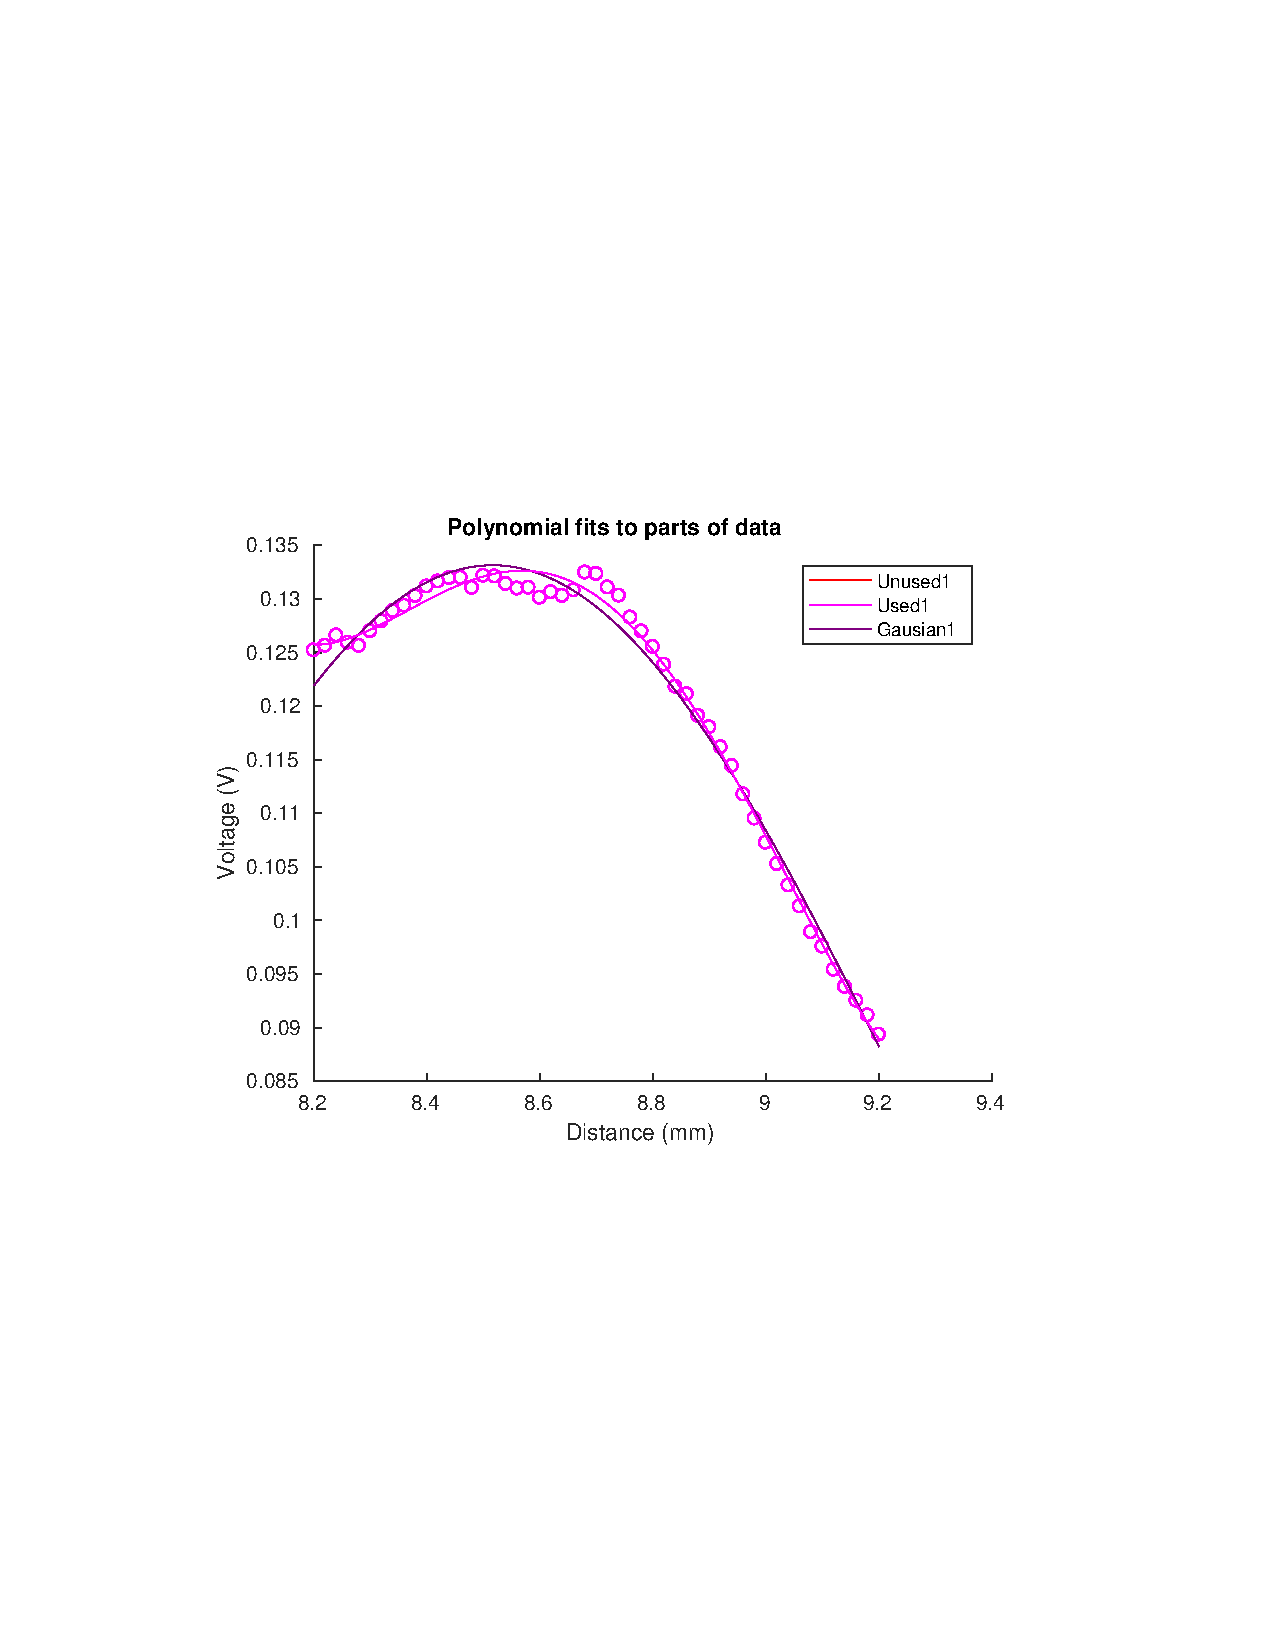
\includegraphics[height=.5\textheight, trim={4cm 8.5cm 4cm 8.5cm},clip]{/home/krg/ESIS_VisEUV_transfer_sw/Output/VIS/grating_1/20170814-135521/iterations/iteration_3/all_fig_combo.pdf}\\
\end{figure}
\end{document}
